
\documentclass{beamer}
\usecolortheme{dove}
\setbeamertemplate{navigation symbols}{}
\usepackage{amsmath,amssymb,amsfonts,amsthm, multicol, subfigure, color}
\usepackage{bm}
\usepackage{graphicx}
\usepackage{tabularx}
\usepackage{booktabs}
\usepackage{hyperref}
\usepackage{pdfpages}
\usepackage{xcolor}
\definecolor{seagreen}{RGB}{46, 139, 87}
\def\independenT#1#2{\mathrel{\rlap{$#1#2$}\mkern2mu{#1#2}}}
\newcommand\indep{\protect\mathpalette{\protect\independenT}{\perp}}
\def\log{\text{log}}
\newcommand\logit{\text{logit}}
\newcommand\iid{\stackrel{\text{iid}}{\sim}}
\newcommand\E{\text{E}}
\newcommand\V{\text{V}}
\renewcommand\P{\text{P}}
\newcommand{\Cov}{\text{Cov}}
\newcommand{\Cor}{\text{Cor}}
\newcommand\doop{\texttt{do}}
\usepackage{stackrel}
\usepackage{tikz}
\usetikzlibrary{arrows,shapes.arrows,positioning,shapes,patterns,calc}
\newcommand\slideref[1]{\vskip .1cm \tiny \textcolor{gray}{{#1}}}
\newcommand\red[1]{\color{red}#1}
\newcommand\blue[1]{\color{blue}#1}
\newcommand\gray[1]{\color{gray}#1}
\newcommand\seagreen[1]{\color{seagreen}#1}
\newcommand\purple[1]{\color{purple}#1}
\newcommand\orange[1]{\color{orange}#1}
\newcommand\black[1]{\color{black}#1}
\newcommand\white[1]{\color{white}#1}
\newcommand\teal[1]{\color{teal}#1}
\newcommand\magenta[1]{\color{magenta}#1}
\newcommand\Fuchsia[1]{\color{Fuchsia}#1}
\newcommand\BlueGreen[1]{\color{BlueGreen}#1}
\newcommand\bblue[1]{\textcolor{blue}{\textbf{#1}}}
\newcommand\bred[1]{\textcolor{red}{\textbf{#1}}}
\newcommand\bgray[1]{\textcolor{gray}{\textbf{#1}}}
\newcommand\bgreen[1]{\textcolor{seagreen}{\textbf{#1}}}
\newcommand\bref[2]{\href{#1}{\color{blue}{#2}}}
\colorlet{lightgray}{gray!40}
\pgfdeclarelayer{bg}    % declare background layer for tikz
\pgfsetlayers{bg,main} % order layers for tikz
\newcommand\mycite[1]{\begin{scriptsize}\textcolor{darkgray}{(#1)}\end{scriptsize}}
\newcommand{\tcframe}{\frame{
%\small{
\only<1|handout:0>{\tableofcontents}
\only<2|handout:1>{\tableofcontents[currentsubsection]}}
%}
}

\usepackage[round]{natbib}
\bibliographystyle{humannat-mod}
\setbeamertemplate{enumerate items}[default]
\usepackage{mathtools}
\usepackage{ulem}

% Need to add examples

\newcommand{\goalsframe}{\begin{frame}{Learning goals for today}
At the end of class, you will be able to:
\begin{enumerate}
\item Understand how linear path models are like DAGs, but with additional statistical assumptions
\item Determine the covariance between standardized variables using a linear path model
\end{enumerate} \vskip .2in
Despite their historical importance in quantitative social science,\\in many applications linear path models are not as useful as DAGs\\because the linear parametric assumptions may not hold.
\end{frame}}

\title{From DAGs to linear path models}
\author{Ian Lundberg}
\date{Soc 212C}

\begin{document}

\maketitle

\goalsframe

\begin{frame}{We have been working with DAGs}

\begin{center}
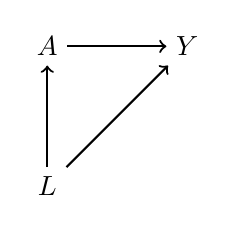
\begin{tikzpicture}[x = .7in, y = .7in]
\node (l) at (0,-1) {$L$};
\node (a) at (0,0) {$A$};
\node (y) at (1,0) {$Y$};
\draw[->, thick] (l) -- (a);
\draw[->, thick] (a) -- (y);
\draw[->, thick] (l) -- (y);
\end{tikzpicture}
\end{center}

\begin{itemize}
\item Each node is a variable
\item Each edge is a direct causal effect
\item The DAG is nonparametric
\begin{itemize}
\item Effect of $A$ may be nonlinear
\item Effect of $A$ may be heterogeneous across $L$
\end{itemize}
\end{itemize} \vskip .1in
$$\E(Y\mid A, L) = f(A,L) \qquad \leftarrow \text{arbitrarily complex }f()$$

\end{frame}

\begin{frame}{Today we will use linear path models} \pause

\begin{center}
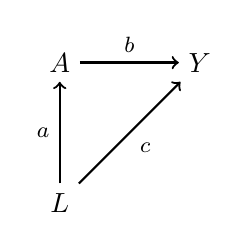
\begin{tikzpicture}[x = .7in, y = .7in]
\node (l) at (0,-1) {$L$};
\node (a) at (0,0) {$A$};
\node (y) at (1,0) {$Y$};
\draw[->, thick] (l) -- node[midway, left, font = \footnotesize] {$a$} (a);
\draw[->, thick] (a) -- node[midway, above, font = \footnotesize] {$b$} (y);
\draw[->, thick] (l) -- node[midway, below right, font = \footnotesize] {$c$} (y);
\end{tikzpicture}
\end{center} \pause

Adds a \bgray{parametric assumption:}\\
Each output is a linear, additive function of its inputs \pause
$$\E(Y\mid A, L) = \alpha + bA + cL$$ \pause \vspace{-.2in}
\begin{itemize}
\item Homogeneous causal effects \pause
\item Linear causal effects \pause
\end{itemize}
\vskip .1in
We will also assume all variables are \bgray{standardized}\\to mean 0 and variance 1

\end{frame}

\begin{frame}

\centering
\includegraphics[height = \textheight]{figs/wright1921_p1}

\end{frame}

\begin{frame}{Wright's (1921) path rule:\\Connecting causal paths to statistical associations}

\begin{center}
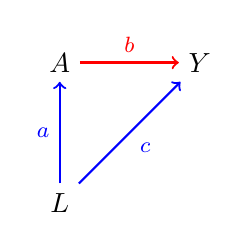
\begin{tikzpicture}[x = .7in, y = .7in]
\node (l) at (0,-1) {$L$};
\node (a) at (0,0) {$A$};
\node (y) at (1,0) {$Y$};
\draw[->, thick, red] (a) -- node[midway, above, font = \footnotesize] {$b$} (y);
\draw[->, thick, blue] (l) -- node[midway, left, font = \footnotesize] {$a$} (a);
\draw[->, thick, blue] (l) -- node[midway, below right, font = \footnotesize] {$c$} (y);
\end{tikzpicture}
\end{center} 

$$\Cov(A,Y) = \textcolor{red}{b} + \textcolor{blue}{ac}$$

\bgray{Wright's rule:}\\When all variables are standardized to variance 1,\\the covariance between two variables\\is the sum over unblocked paths\\of the product of coefficients on that path

\end{frame}

% outtake quick practice

\begin{frame}[t]{When is Wright's rule helpful? Reasoning about biases}

\begin{center}
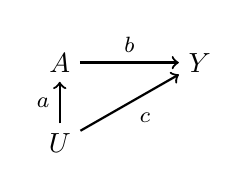
\begin{tikzpicture}[x = .7in, y = .4in]
\node (l) at (0,-1) {$U$};
\node (a) at (0,0) {$A$};
\node (y) at (1,0) {$Y$};
%\node (ytilde) at (1,-1) {$\tilde{Y}$};
\draw[->, thick] (l) -- node[midway, left, font = \footnotesize] {$a$} (a);
\draw[->, thick] (a) -- node[midway, above, font = \footnotesize] {$b$} (y);
\draw[->, thick] (l) -- node[midway, below right, font = \footnotesize] {$c$} (y);
%\draw[->, thick] (y) -- node[midway, right, font = \footnotesize] {$\eta_{Y\tilde{Y}}$} (ytilde);
\end{tikzpicture}
\end{center} 

Suppose we don't observe $U$. \pause We regress $Y$ on $A$.
$$\E(Y\mid A) = \alpha + \beta A$$ \pause
What do we get? \pause
$$\begin{aligned}
\beta &= \frac{\Cov(A,Y)}{\V(Y)} &\text{from regression} \\ \pause
&= \Cov(A,Y) &\text{since standardized} \\ \pause
&= \underbrace{b}_\text{Estimand} + \underbrace{ac}_\text{Bias} &\text{Wright's rule}
\end{aligned}$$

\end{frame}

\begin{frame}{Why you should rarely use linear path models}

\begin{enumerate}
\item DAGs formalize causal beliefs
\begin{itemize}
\item good for human reasoning
\item not very amenable to machine learning
\end{itemize}
\item Nonlinear statistical patterns can be learned from data
\begin{itemize}
\item hard for humans to reason about
\item easy to plug in machine learning
\end{itemize}
\end{enumerate} \vskip .15in

DAGs + ML separate (1) and (2)\\
Linear path models lump them together

\end{frame}

\end{document}

